\section{QSIMON}

\begin{frame}{QSIMON\footfullcite{gos}}
\begin{itemize}
    \item The path for $i^{th}$ bit from $R_0$ which can be written as
    \pause
\begin{center}
    \begin{equation*}
    R_2(i) = L_1(i) = R_0(i) \oplus (L_0(i+1)mod(n) \wedge L_0(i+8)mod(n)) \oplus \\
    \hspace{4cm}L_0(i+2)mod(n) \oplus k_0
\end{equation*}
\end{center}
\pause
\item Use the qubits of $R_0$ for storing $L_1$ and $L_0$ becomes $R_1$. This eliminates the need for ancilla qubits.
\pause
\item For computing $R_2(i)$, we can use the following operations:
\begin{enumerate}
    \item CCX($L_0(i+1)mod(n), L_0(i+8)mod(n), R_0(i)$)
    \item CX($L_0(i+2)mod(n), R_0(i)$)
    \item CX($k_0(i), R_0(i)$)
\end{enumerate}
\pause
\item $n$ Toffoli gates and $2n$ CNOT gates for a single round.
\end{itemize}
\end{frame}
\begin{frame}{QSIMON Contd.}
    Define three functions that together form one round of the QSIMON.
    \begin{figure}[h!]
\minipage{0.32\textwidth}
   
   \resizebox{4cm}{!}{
   \begin{quantikz}
    \lstick{$\ket{b}$} &[2mm] \ctrl{1} & \qw & \rstick{$\ket{b}$} \qw  \\
    \lstick{$\ket{a}$} &[2mm] \gate{F} & \qw & \rstick{$\ket{a\oplus S^1(b)S^8(b)}$} \qw \\
    \end{quantikz}
    }
\endminipage\hfill
\minipage{0.32\textwidth}
  \resizebox{4cm}{!}{
   \begin{quantikz}
    \lstick{$\ket{b}$} &[2mm] \ctrl{1} & \qw & \rstick{$\ket{b}$} \qw  \\
    \lstick{$\ket{a}$} &[2mm] \gate{G} & \qw & \rstick{$\ket{a\oplus S^2(b)}$} \qw \\
    \end{quantikz}
    }
\endminipage\hfill
\minipage{0.32\textwidth}%
 \resizebox{4cm}{!}{
   \begin{quantikz}
    \lstick{$\ket{b}$} &[2mm] \ctrl{1} & \qw & \rstick{$\ket{b}$} \qw  \\
    \lstick{$\ket{a}$} &[2mm] \gate{H} & \qw & \rstick{$\ket{a\oplus b}$} \qw \\
    \end{quantikz}
    }
\endminipage
\caption{Subroutines for one round of QSIMON}
\label{fig:sqs}
\end{figure}
\pause
\begin{figure}[h!]
    \centering
    \begin{quantikz}
    \lstick{$\ket{k_0}$} &[2mm] \qw & \qw & \ctrl{2} & \rstick{$\ket{k_1}$} \qw  & & &\qw &\qw & \ctrl{1} &\qw & \rstick{$\ket{k_2}$} \qw \\
    \lstick{$\ket{L_0}$} &[2mm] \ctrl{1} & \ctrl{1} & \qw & \rstick{$\ket{R_1}$} \qw & & & \gate{F} & \gate{G} &\gate{H} &\qw & \rstick{$\ket{L_2}$} \qw  \\
    \lstick{$\ket{R_0}$} &[2mm] \gate{F} & \gate{G} & \gate{H} & \qw \rstick{$\ket{L_1}$} & & & \ctrl{-1} & \ctrl{-1} &\qw &\qw & \rstick{$\ket{R_2}$} \qw   \\
    \end{quantikz}
    \caption{2 Round of QSIMON}
    \label{fig:2rqs}
\end{figure}
\end{frame}
\begin{frame}{Key Expansion}
    Define a function as 
\begin{equation*}
    R_q(a,b) = (S^{-i}(b)\oplus a, b)
\end{equation*}
\pause
This function will be used in the circuit of key expansion.
\begin{figure}[h!]
    \centering
    \begin{quantikz}
    \lstick{$\ket{b}$} &[2mm] \ctrl{1} & \qw & \rstick{$\ket{b}$} \qw  \\
    \lstick{$\ket{a}$} &[2mm] \gate{R_q} & \qw & \rstick{$\ket{(S^{-i}(b)\oplus a}$} \qw \\
    \end{quantikz}
    \caption{Quantum circuit for $R_q(a,b)$}
    \label{fig:keeqs}
\end{figure}
\pause
Case for $m=2$.
\begin{figure}[h!]
    \centering
    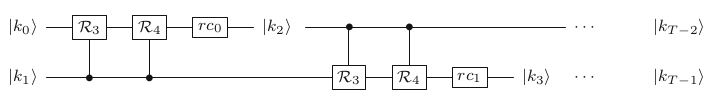
\includegraphics[width=\linewidth]{simon/m2.png}
    \caption{Key expansion for m = 2 \cite{gos}}
    \label{fig:kem2}
\end{figure}
\end{frame}
\begin{frame}{QSIMON (m = 2)}
    \begin{figure}[h!]
    \centering
    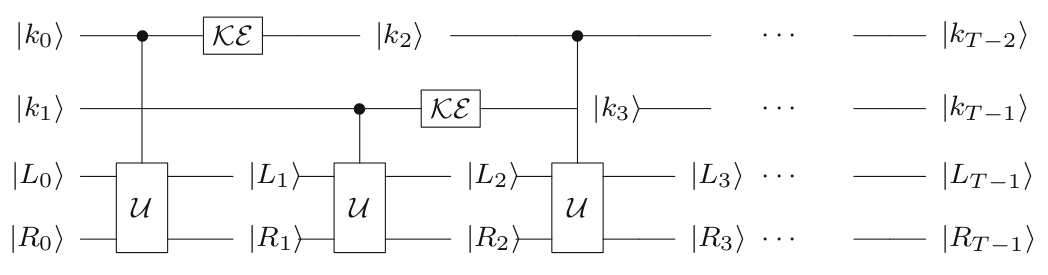
\includegraphics[width=\linewidth]{simon/qsim2.png}
    \caption{QSIMON for m = 2 \cite{gos}}
    \label{fig:qsim2}
\end{figure}
\end{frame}
\begin{frame}{Grover's Attack}
    \begin{figure}[h!]
    \centering
    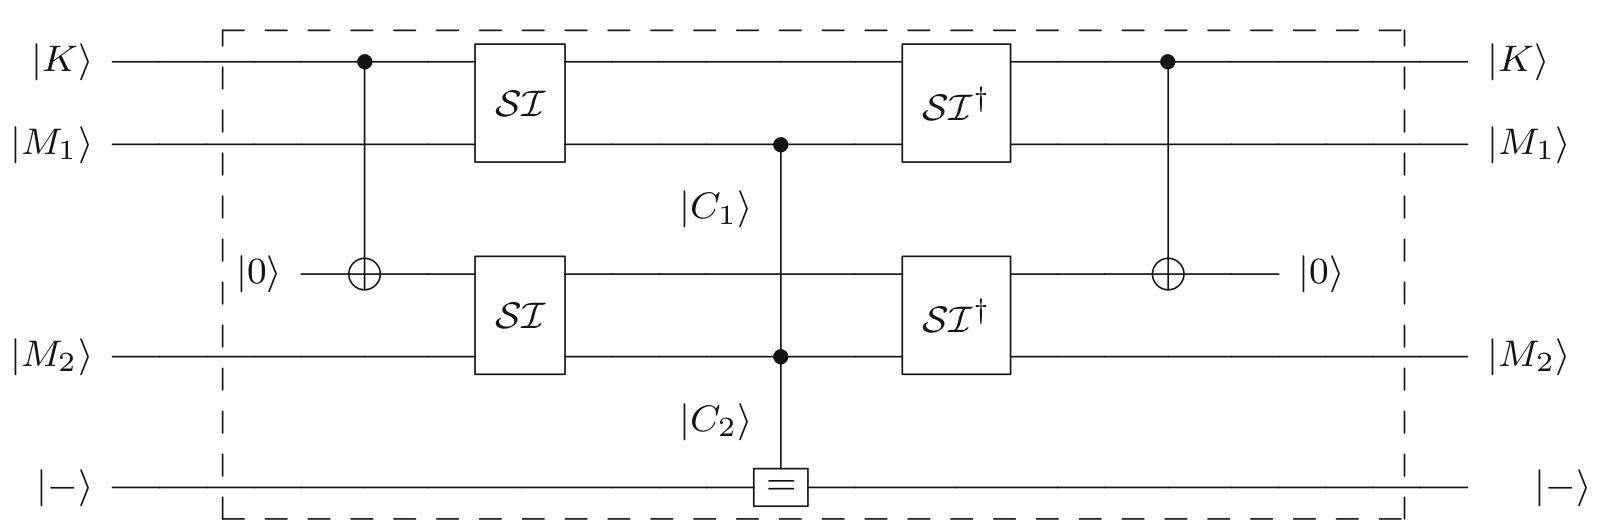
\includegraphics[width=\linewidth]{simon/qsimgrov.png}
    \caption{Grover's Attack on QSIMON \cite{gos}}
    \label{fig:qsimgrov}
\end{figure}
\begin{itemize}
    \item For finding unique key we need r = 2.
    \pause
    \item  In general, we require $2nr$ qubits for messasges and $mn$ qubits for master key.
    \pause
    \item $O(mn + 2nr)$.
\end{itemize}
\end{frame}